\documentclass[12pt]{article}
\usepackage[usenames]{color}
\usepackage{verbatim}
\usepackage{multirow}
\usepackage{fancyhdr}
\usepackage{graphicx}
\usepackage{amssymb,amsthm}
\usepackage{amsmath}
\usepackage[dvipsnames]{xcolor}
\usepackage[left=1in,top=1in,right=1in,bottom=1in,letterpaper]{geometry}
\renewcommand{\baselinestretch}{1.2}
\newcommand{\Cx}{\mathbb{C}}
\usepackage{dirtytalk}
\usepackage{hyperref}
\usepackage{pgfplots}
\pgfplotsset{width=10cm,compat=1.9}
\pagestyle{plain}
\lhead{}
\chead{}
\rhead{}
\lfoot{}
\cfoot{\thepage}
\rfoot{}
\renewcommand{\headrulewidth}{0.4pt}
\renewcommand{\footrulewidth}{0.4pt}
\renewcommand{\lim}{\mathrm{lim}}
\renewcommand{\ln}{\mathrm{ln}}
\usepackage{mathtools}
\usepackage{amsmath}
\usepackage{amsthm}
\usepackage{mathrsfs}
\usepackage{amssymb}
\usepackage{amsfonts}
\usepackage{subfigure}
\usepackage{multicol}
\usepackage[normalem]{ulem} % to use \sout
\newcommand{\remove}[1]{{\color{Gray}\sout{#1}}}
\newcommand{\revise}[1]{{\color{blue}#1}}
\newcommand{\comm}[1]{{\color{red}(yx: #1)}}
\newcommand{\bm}[1]{\boldsymbol{#1}}
\newcommand{\prev}{{\mathrm{prev}}} % previous iteration
\usepackage{array}
\newcolumntype{L}{>{\centering\arraybackslash}m{2.5cm}}
\DeclareMathOperator{\shrink}{shrink} % shrinkage
\DeclareMathOperator{\hardthr}{hardthr} % hard thresholding
\DeclareMathOperator*{\argmin}{arg\,min} % argmin
\DeclareMathOperator*{\argmax}{arg\,max} % argmax
\DeclareMathOperator*{\Min}{minimize}
\DeclareMathOperator*{\Max}{maximize}
\newcommand{\bc}{\begin{center}}
\newcommand{\ec}{\end{center}}
\newcommand{\bdm}{\begin{displaymath}}
\newcommand{\edm}{\end{displaymath}}
\newcommand{\beq}{\begin{equation}}
\newcommand{\eeq}{\end{equation}}
\newcommand{\bfl}{\begin{flushleft}}
\newcommand{\efl}{\end{flushleft}}
\newcommand{\bt}{\begin{tabbing}}
\newcommand{\et}{\end{tabbing}}
\newcommand{\beqn}{\begin{eqnarray}}
\newcommand{\eeqn}{\end{eqnarray}}
\newcommand{\beqs}{\begin{align*}} 
\newcommand{\eeqs}{\end{align*}}  
\newtheorem{theorem}{Theorem}[section]
\newtheorem{claim}{Claim}[section]
\newtheorem{corollary}{Corollary}[section]
\newtheorem{definition}{Definition}[section]
\newtheorem{example}{Example}[section]
\newtheorem{lemma}{Lemma}[section]
\newtheorem{proposition}{Proposition}[section]
\newtheorem{remark}{Remark}[section]
\newtheorem{assumption}{Assumption}
\newcommand{\hvx}{{\hat{\vx}}}
\DeclarePairedDelimiter{\dotp}{\langle}{\rangle} 
\usepackage[shortlabels]{enumitem}
\usepackage[normalem]{ulem}
\usepackage{float}
\usepackage{listings}

\begin{document}

\noindent {\bf MA103: Data-Driven Modeling}

\noindent {\bf Objective Functions and Solving}
\vspace{.5em}
\hrule \hrule
\vspace{.5em}

\noindent So far we've focused on constraint formulation, let's shift focus to the objective and solving our linear programs. We'll start with a familiar problem:\\

\noindent \textbf{Wyndor}  The Wyndor Glass Co. produces high-quality glass products, including windows and glass doors. The company has three plants that simultaneously produce the components of its products. Doors require one hour of production time at Plant 1 and three hours of production time at Plant 3. Windows require two hours each at Plants 2 and 3. Plant 1 has 4 hours available each week, Plant 2 has 12 hours available each week, and Plant 3 has 18 hours available each week.\par \vspace{9pt} 
    
\noindent If Wyndor makes \$300 on each door they sell and \$500 on each window they sell, how many windows and doors should Wyndor Glass Co. produce each week to maximize profit?\par \vspace{9pt} 

\noindent We are familiar with the feasible region of the Wyndor problem from our reading, but how do we know what the optimal solution is? Let's take some time today to consider the objective function.

\begin{minipage}[c]{0.38\textwidth}
\textbf{Formulate a Linear Program:}
\[
\begin{aligned}
\max \quad & z = 300x_1 + 500x_2 \\
\text{s.t.} \quad & x_1 \le 4 \\
& 2x_2 \le 12 \\
& 3x_1 + 2x_2 \le 18 \\
& x_1 \ge 0 \\
& x_2 \ge 0
\end{aligned}
\]
\end{minipage}%
\hfill
\begin{minipage}[c]{0.6\textwidth}
\centering
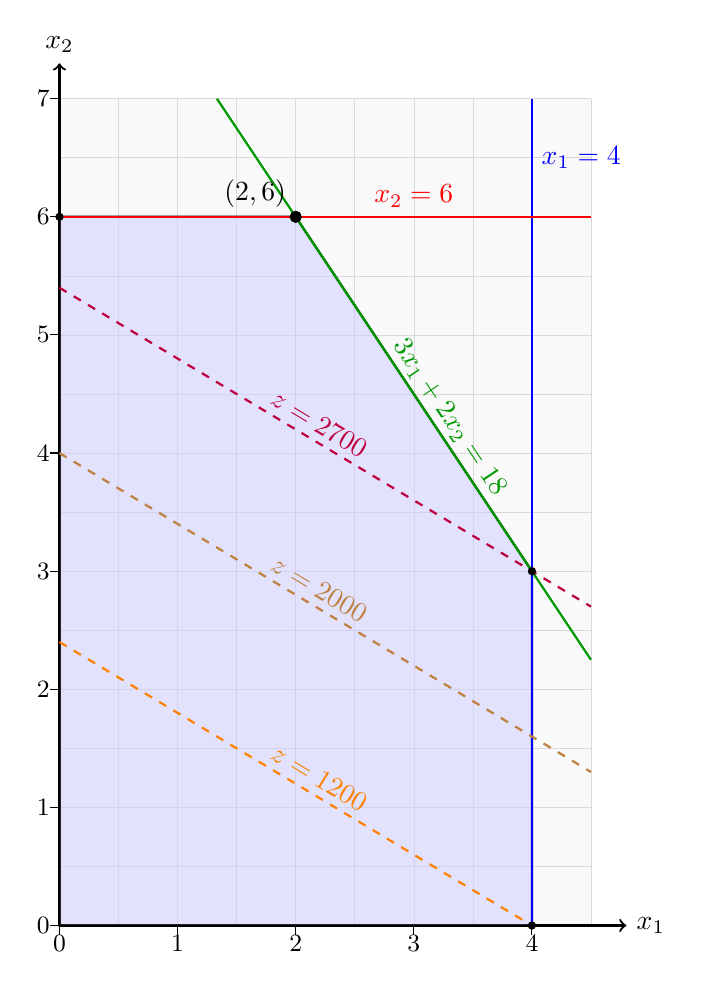
\begin{tikzpicture}[x=1.5cm,y=1.5cm]

% Background
\fill[gray!5] (0,0) rectangle (4.5,7);

% Grid
\draw[step=0.5,gray!30,very thin] (0,0) grid (4.5,7);

% Axes
\draw[->,thick] (0,0) -- (4.8,0)
    node[right] {$x_1$};

\draw[->,thick] (0,0) -- (0,7.3)
    node[above] {$x_2$};

% Tick marks and labels
\foreach \x in {0,1,2,3,4}
{
    \draw (\x,0) -- (\x,-0.08);
    \node[below] at (\x,0) {\small \x};
}

\foreach \y in {0,1,2,3,4,5,6,7}
{
    \draw (0,\y) -- (-0.08,\y);
    \node[left] at (0,\y) {\small \y};
}

% Feasible region
\fill[blue!20,opacity=.5]
    (0,0) --
    (4,0) --
    (4,3) --
    (2,6) --
    (0,6) --
    cycle;

\draw[thick]
    (0,0) --
    (4,0) --
    (4,3) --
    (2,6) --
    (0,6) --
    cycle;

% Constraint x1 = 4
\draw[blue,thick] (4,0) -- (4,7);
\node[blue,right] at (4,6.5)
    {$x_1=4$};

% Constraint x2 = 6
\draw[red,thick] (0,6) -- (4.5,6);
\node[red,above] at (3,6)
    {$x_2=6$};

% Constraint 3x1 + 2x2 = 18
\draw[green!60!black,thick]
    (4/3,7) -- (4.5,2.25);

\node[
    green!60!black,
    fill=none,
    inner sep=1pt,
    rotate=-56
] at (3.3,4.3)
{$3x_1+2x_2=18$};

% Level curve z = 1200
\draw[dashed,orange,thick]
    (0,2.4) -- (4,0);

\node[
    orange,
    fill=none,
    inner sep=1pt,
    rotate=-31
] at (2.2,1.25)
{$z=1200$};

% Level curve z = 2000
\draw[dashed,brown,thick]
    (0,4) -- (4.5,1.3);

\node[
    brown,
    fill=none,
    inner sep=1pt,
    rotate=-31
] at (2.2,2.85)
{$z=2000$};

% Level curve z = 2700
\draw[dashed,purple,thick]
    (0,5.4) -- (4.5,2.7);

\node[
    purple,
    fill=none,
    inner sep=1pt,
    rotate=-31
] at (2.2,4.25)
{$z=2700$};

% Vertices
\fill (4,0) circle (1.5pt);
\fill (4,3) circle (1.5pt);
\fill (2,6) circle (1.5pt);
\fill (0,6) circle (1.5pt);

% Optimal solution
\filldraw[black] (2,6) circle (2pt);
\node[above left] at (2,6)
    {$(2,6)$};

\end{tikzpicture}
\end{minipage}

\newpage
\begin{enumerate}
    \item What do the dashed lines at $z=1200$, $z=2000$, and $z=2700$ represent on the feasible region plot? What do we call these curves? How do they help us find the optimal solution? \vfill
    \item How many variables are in the objective function? Does this function represent a line in two dimensional space? What else could it represent?\vfill
    \item Place your shape on top of the Wyndor feasible region. Where is the optimal solution? Where would the optimal solution be if this was a minimization problem? \vfill
    \item What do you notice about the location of the optimal solution? \vfill
    \item What problem might you encounter if the proportionality assumption of linear programming did not hold in our objective function? \vfill
\end{enumerate}
\newpage
\noindent \textbf{The Engineer Problem.} Your Engineer Platoon has 2 different MOS types: 12B and 12N. 12B Soldiers are combat engineers, 12Ns are heavy equipment operators. You’re preparing a defense against an enemy Armored Company. There are two types of obstacles you can build: an Anti-Tank Ditch (ATD) and an 11-Row wire obstacle. The ATD requires 3 x 12N Soldiers and 1 x 12B Soldier. The 11-Row requires 1 x 12N and 2 x 12Bs. You only have 9 x 12Ns and 8 x 12Bs. Each ATD will span 300 meters and the 11 Row will block 200 meters. How many of each type should your Platoon build to maximize the amount of perimeter (in meters) you can protect?\\

\begin{equation} \label{dual_SVM}
\begin{aligned}
\max_{x_1,x_2} \quad & P=300x_1+200x_2 \\
\textrm{s.t.} \quad & 3x_1+x_2\leq 9\\ 
& x_1+2x_2\leq 8 \\
& x_1, x_2\geq 0\\
\end{aligned}
\end{equation}

\noindent As with the Wyndor problem, we know what the feasible region looks like for this problem, but how do we find the optimal solution?\\

\noindent Visualizing the objective function:

\begin{minipage}[t]{0.48\textwidth}

    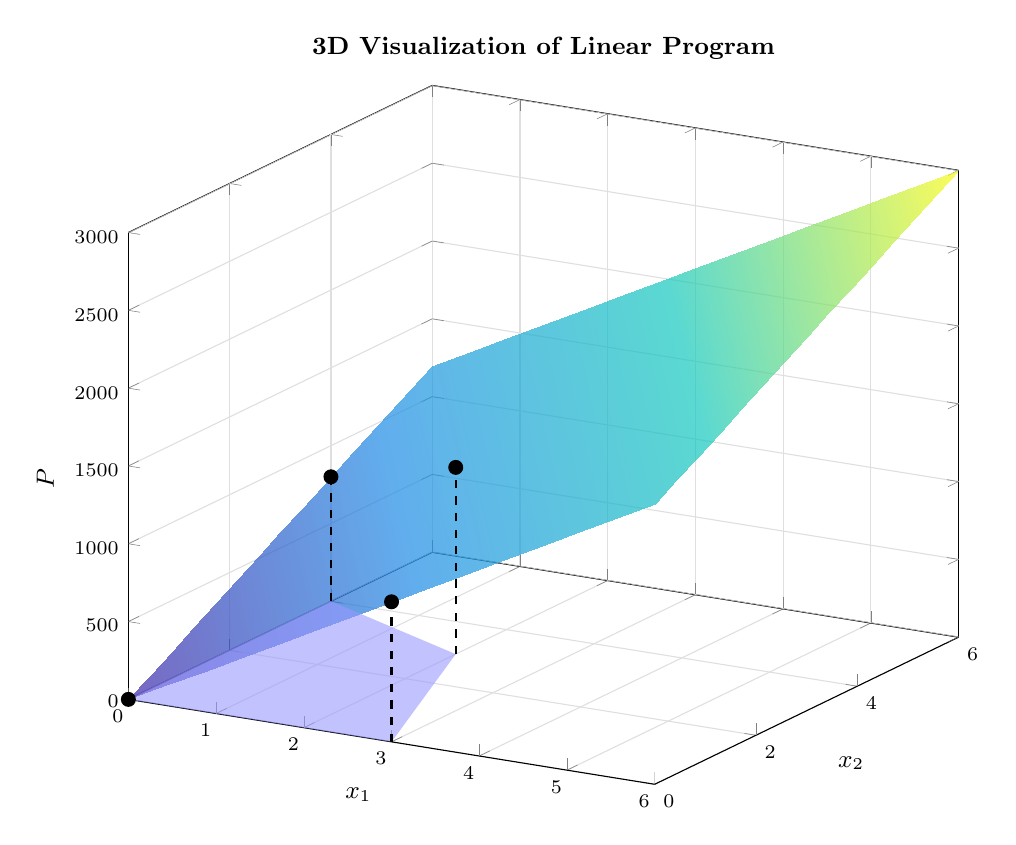
\begin{tikzpicture}
    \begin{axis}[
    width=\linewidth,
    view={30}{20},
    title={\textbf{3D Visualization of Linear Program}},
    xlabel={$x_1$}, ylabel={$x_2$}, zlabel={$P$},
    xmin=0, xmax=6, ymin=0, ymax=6, zmin=0, zmax=3000,
    xtick={0,...,6}, ytick={0,2,4,6},
    ztick={0,500,...,3000},
    scaled z ticks=false,
    zticklabel style={/pgf/number format/1000 sep={}},
    grid=major, grid style={gray!25},
    tick label style={font=\scriptsize},
    label style={font=\small},
    title style={font=\small},
    colormap={parula}{rgb255=(62,38,168) rgb255=(30,140,230) rgb255=(20,200,190) rgb255=(250,250,20)},
]
% Objective plane P = 300x1 + 200x2
\addplot3[surf, shader=interp, opacity=0.7, domain=0:6, y domain=0:6, samples=15]
    {300*x + 200*y};
% Feasible region on the floor
\addplot3[fill=blue!40, fill opacity=0.6, draw=none]
    coordinates {(0,0,0) (3,0,0) (2,3,0) (0,4,0) (0,0,0)};
% Dashed lines from corner points up to the plane
\addplot3[black, thick, dashed] coordinates {(3,0,0) (3,0,900)};
\addplot3[black, thick, dashed] coordinates {(2,3,0) (2,3,1200)};
\addplot3[black, thick, dashed] coordinates {(0,4,0) (0,4,800)};
% Corner points on the plane
\addplot3[only marks, mark=*, mark size=2.5pt, black]
    coordinates {(0,0,0) (3,0,900) (2,3,1200) (0,4,800)};
\end{axis}
\end{tikzpicture}
\end{minipage}
\hfill
\begin{minipage}[t]{0.48\textwidth}
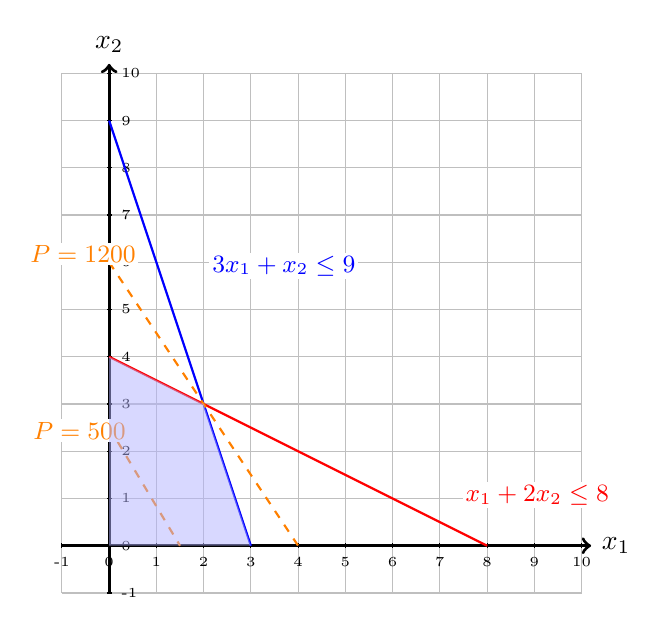
\begin{tikzpicture}[scale=0.6]

    % Grid and axes
    \draw[gray!50, thin, step=1] (-1,-1) grid (10,10);
    \draw[very thick,->] (-1,0) -- (10.2,0) node[right] {$x_1$};
    \draw[very thick,->] (0,-1) -- (0,10.2) node[above] {$x_2$};

    % Axis ticks
    \foreach \x in {-1,...,10} \draw (\x,0.05) -- (\x,-0.05) node[below] {\tiny\x};
    \foreach \y in {-1,...,10} \draw (-0.05,\y) -- (0.05,\y) node[right] {\tiny\y};

% Inequality 1: 3x + y <= 9 → y = 9 - 3x
\draw[thick,blue] (0,9) -- (3,0) 
    node[pos=0.7, above right, xshift=0pt, yshift=50pt, fill=white, inner sep=1pt] {\small$3x_1 + x_2 \le 9$};

% Inequality 2: x + 2y <= 8 → y = (8 - x)/2
\draw[thick,red] (0,4) -- (8,0) 
    node[pos=0.6, below left, xshift=100pt, yshift=-4pt, fill=white, inner sep=1pt] {\small$x_1 + 2x_2 \le 8$};

% Objective function: 300x + 200y = P → y = (P - 300x)/200
% Dashed line for P = 500
\draw[dashed, thick, orange]
    (0,2.5) -- (1.5,0)
    node[pos=0.6, above left, xshift=-8pt, yshift=20pt, fill=white, inner sep=1pt] {\small$P=500$};


% Solid line for P = 1200
\draw[dashed, thick, orange]
    (0,6) -- (4,0)
    node[pos=0.6, above left, xshift=-30pt, yshift=60pt, fill=white, inner sep=1pt] {\small$P=1200$};

    % Feasible region fill (bounded by the intersection and axes)
    \fill[blue!30,opacity=0.5]
        (0,0) --
        (0,4) -- % y-intercept of blue line
        (2,3) -- % intersection point
        (3,0) -- % x-intercept of red line
        cycle;

\end{tikzpicture}
\end{minipage}

\noindent What did you notice about the location of the optimal solution in the Wyndor problem? Do you notice something similar in the Engineer Problem? Do you think this will always be the case?
\vspace{2cm}

\end{document}